\documentclass[11pt, a4paper]{article}
\usepackage[utf8]{inputenc}
\usepackage[T1]{fontenc}
\usepackage{lmodern}
\usepackage[margin=2.5cm]{geometry}
\usepackage{graphicx}
\usepackage{booktabs}
\usepackage{amsmath}
\usepackage{float}

\graphicspath{{../plotting/}}
\setlength{\parindent}{0pt}
\setlength{\parskip}{6pt}
\setlength{\emergencystretch}{3em}
\setlength{\belowcaptionskip}{6pt}

% ---------------------------------------------------------------------------
% TODO before submission: group name, team members, contribution table
\newcommand{\groupname}{\textbf{[group name]}}
\newcommand{\groupmembers}{Laurent~Stuck, \textbf{[name 2]}, \textbf{[name 3]}, \textbf{[name 4]}}
% ---------------------------------------------------------------------------

\begin{document}

{\Large \textbf{Robotics: Assignment 2}}

Group \groupname: \\
\groupmembers

\section*{Abbreviations}

\begin{gather*}
  s_i = \sin(q_i), \quad c_i = \cos(q_i), \quad
  s_{ij} = \sin(q_i + q_j), \quad c_{ij} = \cos(q_i + q_j), \\
  s_{123} = \sin(q_1 + q_2 + q_3), \quad c_{123} = \cos(q_1 + q_2 + q_3)
\end{gather*}

$L_1 = 0.4318 - 0.0203 = 0.41$\,m, $L_2 = 0.43$\,m and $L_3 = 0.055$\,m are the link lengths from
\texttt{forwardkinematics.hpp} (\texttt{l1}, \texttt{l2}, \texttt{l3} in the code).
All angles are in radians. ${}^{i-1}_{\;\;i}T$ is the homogeneous transformation from frame $i-1$ to frame $i$.

% ===========================================================================
\section*{A: Forward Kinematics}

\subsection*{Task 1: DH parameters}

We use the DH convention from the tutorial (Craig). The four parameters are read off Fig.~1 of the
assignment sheet with these definitions:

\begin{itemize}
  \item $\alpha_{i-1}$: angle from $z_{i-1}$ to $z_i$, measured about $x_{i-1}$
  \item $a_{i-1}$: distance from $z_{i-1}$ to $z_i$, measured along $x_{i-1}$
  \item $d_i$: distance from $x_{i-1}$ to $x_i$, measured along $z_i$
  \item $\theta_i$: angle from $x_{i-1}$ to $x_i$, measured about $z_i$
\end{itemize}

\begin{table}[H]
  \centering
  \caption{DH parameters for the 3-DoF RRR Puma}
  \begin{tabular}{c c c c c}
    \toprule
    $i$ & $\alpha_{i-1}$ & $a_{i-1}$ & $d_i$ & $\theta_i$ \\
    \midrule
    1    & 0 & 0     & 0 & $q_1$ \\
    2    & 0 & $L_1$ & 0 & $q_2 - \frac{\pi}{2}$ \\
    3    & 0 & $L_2$ & 0 & $q_3$ \\
    4(E) & 0 & $L_3$ & 0 & 0 \\
    \bottomrule
  \end{tabular}
\end{table}

How we got the entries:

\begin{itemize}
  \item $\alpha_{i-1} = 0$ in every row: the arm is planar, so all joint axes ($z$ axes) are parallel.
  \item $d_i = 0$ in every row: all frames lie in the same plane, there is no offset along $z$.
  \item $a_{i-1}$ is the distance between two neighbouring joint axes, which is the length of the link
        between them. Frames 0 and 1 have the same origin, therefore $a_0 = 0$.
  \item $\theta_i$ contains the joint angle, because all joints are revolute. In row 2 there is an
        additional constant offset of $-\frac{\pi}{2}$: in the zero configuration $x_1$ points to the right and
        $x_2$ points up. In Fig.~1 $x_0$ points to the right and $y_0$ points down, so $z$ points into the
        drawing plane and positive angles turn clockwise. Turning from ``right'' to ``up'' is
        counter-clockwise, which gives the negative sign.
  \item There is no joint between frame 3 and the end effector frame E. E has the same orientation
        as frame 3, so $\theta_4 = 0$.
\end{itemize}

\texttt{computeDH()} writes exactly this table into \texttt{DH}, one row per frame, with the current
joint angles \texttt{angles[0..2]}.

\subsection*{Task 2: Transformation between frames}

The general transformation between two frames from the DH parameters is (tutorial, Craig p.~74):
\[
  {}^{i-1}_{\;\;i}T =
  \begin{pmatrix}
    c\theta_i & -s\theta_i & 0 & a_{i-1} \\
    s\theta_i\, c\alpha_{i-1} & c\theta_i\, c\alpha_{i-1} & -s\alpha_{i-1} & -s\alpha_{i-1}\, d_i \\
    s\theta_i\, s\alpha_{i-1} & c\theta_i\, s\alpha_{i-1} & c\alpha_{i-1} & c\alpha_{i-1}\, d_i \\
    0 & 0 & 0 & 1
  \end{pmatrix}
\]

\textbf{Simplification:} in our table $\alpha_{i-1} = 0$ and $d_i = 0$ in every row, so
$c\alpha_{i-1} = 1$ and $s\alpha_{i-1} = 0$. Every transformation is a rotation about $z$ by $\theta_i$
and a translation by $a_{i-1}$ along $x$:
\[
  {}^{i-1}_{\;\;i}T =
  \begin{pmatrix}
    c\theta_i & -s\theta_i & 0 & a_{i-1} \\
    s\theta_i & c\theta_i & 0 & 0 \\
    0 & 0 & 1 & 0 \\
    0 & 0 & 0 & 1
  \end{pmatrix}
\]

Inserting the four rows of the DH table gives the four matrices. In row 2 we use the identities
$\cos(q_2 - \frac{\pi}{2}) = s_2$ and $\sin(q_2 - \frac{\pi}{2}) = -c_2$.

\[
  {}^0_1T =
  \begin{pmatrix} c_1 & -s_1 & 0 & 0 \\ s_1 & c_1 & 0 & 0 \\ 0 & 0 & 1 & 0 \\ 0 & 0 & 0 & 1 \end{pmatrix}
  \qquad
  {}^1_2T =
  \begin{pmatrix} s_2 & c_2 & 0 & L_1 \\ -c_2 & s_2 & 0 & 0 \\ 0 & 0 & 1 & 0 \\ 0 & 0 & 0 & 1 \end{pmatrix}
\]
\[
  {}^2_3T =
  \begin{pmatrix} c_3 & -s_3 & 0 & L_2 \\ s_3 & c_3 & 0 & 0 \\ 0 & 0 & 1 & 0 \\ 0 & 0 & 0 & 1 \end{pmatrix}
  \qquad
  {}^3_ET =
  \begin{pmatrix} 1 & 0 & 0 & L_3 \\ 0 & 1 & 0 & 0 \\ 0 & 0 & 1 & 0 \\ 0 & 0 & 0 & 1 \end{pmatrix}
\]

The functions \texttt{computeT0\_1()}, \texttt{computeT1\_2()}, \texttt{computeT2\_3()} and
\texttt{computeT3\_E()} implement these four matrices. The additional variables \texttt{c1}, \texttt{s1}, \ldots{} in the code hold the
cosine and sine of the joint angles.

\textbf{Forward kinematics.} The transformation to the end effector is the product
\[
  {}^0_ET = {}^0_1T \; {}^1_2T \; {}^2_3T \; {}^3_ET .
\]
We multiplied step by step and simplified with the angle sum identities
$s_{12} = s_1 c_2 + c_1 s_2$ and $c_{12} = c_1 c_2 - s_1 s_2$ (and the same for $s_{123}$, $c_{123}$):
\begin{align*}
  {}^0_2T = {}^0_1T \; {}^1_2T &=
  \begin{pmatrix}
    c_1 s_2 + s_1 c_2 & c_1 c_2 - s_1 s_2 & 0 & L_1 c_1 \\
    s_1 s_2 - c_1 c_2 & s_1 c_2 + c_1 s_2 & 0 & L_1 s_1 \\
    0 & 0 & 1 & 0 \\ 0 & 0 & 0 & 1
  \end{pmatrix}
  =
  \begin{pmatrix}
    s_{12} & c_{12} & 0 & L_1 c_1 \\
    -c_{12} & s_{12} & 0 & L_1 s_1 \\
    0 & 0 & 1 & 0 \\ 0 & 0 & 0 & 1
  \end{pmatrix}
  \\[6pt]
  {}^0_3T = {}^0_2T \; {}^2_3T &=
  \begin{pmatrix}
    s_{12} c_3 + c_{12} s_3 & c_{12} c_3 - s_{12} s_3 & 0 & L_1 c_1 + L_2 s_{12} \\
    s_{12} s_3 - c_{12} c_3 & s_{12} c_3 + c_{12} s_3 & 0 & L_1 s_1 - L_2 c_{12} \\
    0 & 0 & 1 & 0 \\ 0 & 0 & 0 & 1
  \end{pmatrix}
  \\[6pt]
  &=
  \begin{pmatrix}
    s_{123} & c_{123} & 0 & L_1 c_1 + L_2 s_{12} \\
    -c_{123} & s_{123} & 0 & L_1 s_1 - L_2 c_{12} \\
    0 & 0 & 1 & 0 \\ 0 & 0 & 0 & 1
  \end{pmatrix}
\end{align*}
${}^3_ET$ only shifts by $L_3$ along $x_3$. This adds $L_3$ times the first column of the rotation to the
position and leaves the rotation unchanged:
\[
  \boxed{
  {}^0_ET(q) =
  \begin{pmatrix}
    s_{123} & c_{123} & 0 & L_1 c_1 + L_2 s_{12} + L_3 s_{123} \\
    -c_{123} & s_{123} & 0 & L_1 s_1 - L_2 c_{12} - L_3 c_{123} \\
    0 & 0 & 1 & 0 \\
    0 & 0 & 0 & 1
  \end{pmatrix}}
\]
\texttt{computeT0\_E()} implements this simplified matrix directly (it does not multiply the four
matrices at run time). The variables \texttt{c12}, \texttt{s12}, \texttt{c123}, \texttt{s123} hold the
cosine and sine of the angle sums.

The result can be read geometrically: all rotations are about the same axis, so the angles add up to
$q_1 + q_2 + q_3 - \frac{\pi}{2}$, and the position is the sum of the three link vectors.

\textbf{Sanity checks.}
\begin{itemize}
  \item $q = (0, 0, 0)^T$: position $(L_1,\, -L_2 - L_3) = (0.41,\, -0.49)$\,m. This is the zero
        configuration of Fig.~1: link 1 points to the right, links 2 and 3 point up. $y$ is negative because
        $y_0$ points down.
  \item $q = (0, \frac{\pi}{2}, 0)^T$: position $(L_1 + L_2 + L_3,\, 0) = (0.90,\, 0)$\,m and the rotation
        part is the identity. The arm is stretched out along $x_0$.
  \item $q = (\frac{\pi}{4}, -\frac{\pi}{4}, \frac{\pi}{4})^T$: position $(0.33,\, -0.18)$\,m.
\end{itemize}

\subsection*{Task 3: End effector position in operational space}

$x$ and $y$ are the first two entries of the last column of ${}^0_ET$ (the translation).
$\alpha$ is the angle of the end effector axis $x_E$ relative to $x_0$, measured about $z_0$. The first
column of the rotation part is $(s_{123},\, -c_{123})^T = (\cos\alpha,\, \sin\alpha)^T$ with
$\alpha = q_1 + q_2 + q_3 - \frac{\pi}{2}$. This is also the sum of the four $\theta_i$ of the DH table.
\[
  \boxed{
  F(q) = \begin{pmatrix} x \\ y \\ \alpha \end{pmatrix} =
  \begin{pmatrix}
    L_1 c_1 + L_2 s_{12} + L_3 s_{123} \\
    L_1 s_1 - L_2 c_{12} - L_3 c_{123} \\
    q_1 + q_2 + q_3 - \frac{\pi}{2}
  \end{pmatrix}}
\]
\texttt{computeF()} takes $x$ and $y$ from \texttt{T0\_E} and computes $\alpha$ from the joint angles.
The constant \texttt{HALF\_PI} in the code is $\frac{\pi}{2}$.

Sanity checks: $F(0, 0, 0) = (0.41,\, -0.49,\, -1.57)^T$, the end effector points up, which is
$-\frac{\pi}{2}$ from $x_0$ because positive angles turn towards $y_0$ (down).
$F(0, \frac{\pi}{4}, 0) = (0.76,\, -0.35,\, -0.79)^T$.

\subsection*{Task 4: End effector Jacobian}

The Jacobian contains the partial derivatives of $F$ with respect to the joint angles,
$J_{ij} = \partial F_i / \partial q_j$. Row $i$ belongs to a component of $F$ ($x$, $y$, $\alpha$),
column $j$ to joint $j$.

$q_1$ appears in every angle sum, $q_2$ only in $s_{12}$, $c_{12}$, $s_{123}$, $c_{123}$, and $q_3$ only in
$s_{123}$, $c_{123}$. With $\frac{\partial}{\partial q} \sin = \cos$ and
$\frac{\partial}{\partial q} \cos = -\sin$:
\[
  \boxed{
  J(q) = \frac{\partial F(q)}{\partial q} =
  \begin{pmatrix}
    -L_1 s_1 + L_2 c_{12} + L_3 c_{123} & L_2 c_{12} + L_3 c_{123} & L_3 c_{123} \\
    L_1 c_1 + L_2 s_{12} + L_3 s_{123} & L_2 s_{12} + L_3 s_{123} & L_3 s_{123} \\
    1 & 1 & 1
  \end{pmatrix}}
\]
The last row is $(1, 1, 1)$ because every joint turns the end effector by the same angle as the joint
itself. \texttt{computeJ()} implements this matrix.

Sanity check for $q = (0, 0, 0)^T$:
\[
  J = \begin{pmatrix} 0.49 & 0.49 & 0.06 \\ 0.41 & 0 & 0 \\ 1 & 1 & 1 \end{pmatrix}
\]
Joint 3 is $L_3$ below the end effector, so it moves the end effector only along $x_0$ by $L_3$.
Joint 2 is $L_2 + L_3 = 0.49$\,m below the end effector and also moves it only along $x_0$.

\subsection*{Task 5: Understanding the Jacobian matrix and pose singularities}

\subsubsection*{(a) Robot poses and translational velocity vectors}

\begin{figure}[H]
  \centering
  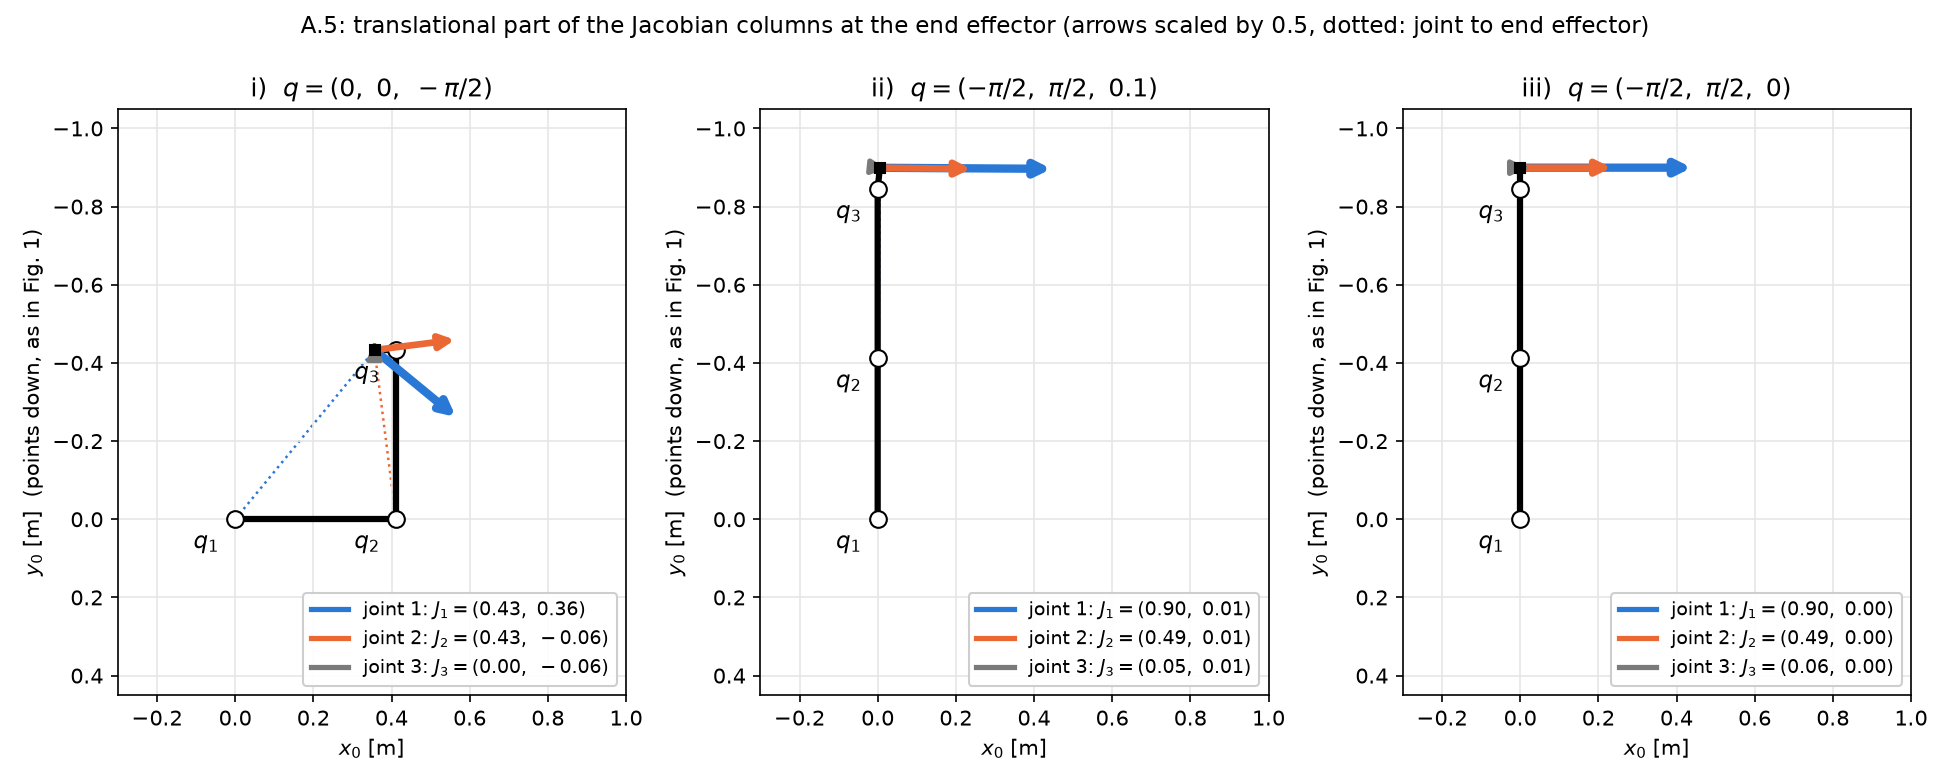
\includegraphics[width=\textwidth]{a5_jacobian.png}
  \caption{Robot pose and the translational part ($x$ and $y$ component) of the three Jacobian columns
  for the three configurations. Axes as in Fig.~1 of the sheet ($y_0$ points down).}
  \label{fig:a5}
\end{figure}

The vectors in Fig.~\ref{fig:a5} are the first two rows of each column of $J$. They agree with the
drawing rule from the tutorial: the vector of joint $j$ is perpendicular to the line from joint $j$ to
the end effector (dotted), its length is the length of this line, and it points in the direction of a
positive joint rotation (clockwise in the figure).

\begin{table}[H]
  \centering
  \caption{Translational velocity vectors $(\partial x / \partial q_j,\ \partial y / \partial q_j)$ in m/rad}
  \begin{tabular}{l c c c}
    \toprule
    Configuration & Joint 1 & Joint 2 & Joint 3 \\
    \midrule
    i. $q = (0, 0, -\frac{\pi}{2})$ & $(0.43,\ 0.36)$ & $(0.43,\ -0.06)$ & $(0,\ -0.06)$ \\
    ii. $q = (-\frac{\pi}{2}, \frac{\pi}{2}, 0.1)$ & $(0.90,\ 0.01)$ & $(0.49,\ 0.01)$ & $(0.05,\ 0.01)$ \\
    iii. $q = (-\frac{\pi}{2}, \frac{\pi}{2}, 0)$ & $(0.90,\ 0)$ & $(0.49,\ 0)$ & $(0.06,\ 0)$ \\
    \bottomrule
  \end{tabular}
\end{table}

\subsubsection*{(b) Singularities}

\begin{itemize}
  \item \textbf{i: fully controllable.} The vectors of joint 1 and joint 2 point in clearly different
        directions. By combining them the end effector can move in every direction of the plane. Joint 3
        hardly moves the end effector but turns it, so the orientation can be chosen as well.
  \item \textbf{ii: close to a singularity.} The arm is almost stretched out. The three vectors are
        almost parallel (all nearly along $x_0$), their components along the arm ($y_0$) are only
        0.01\,m/rad. A velocity along the arm is still possible, but it needs very large joint
        velocities.
  \item \textbf{iii: in a singularity.} The arm is completely stretched out and all three vectors are
        exactly parallel. No combination of joint velocities produces a velocity along the arm ($y_0$).
        The end effector has lost one degree of freedom.
\end{itemize}

In general: if the vectors span the whole plane, the end effector can move in every direction. The more
parallel they become, the closer the robot is to a singularity. If all of them are parallel, the robot
is in a singularity.

\emph{Our own additional check:} a singularity can also be detected with the determinant (lecture).
For our Jacobian $\det J = -L_1 L_2 c_2$. It is $-0.18$ for configuration i and $0$ for
iii. It is also $0$ for ii, because $q_2 = \frac{\pi}{2}$ there as well: links 1 and 2 are
aligned, so the small velocity along the arm in ii comes only from turning link 3 and cannot be chosen
independently of the orientation $\alpha$. For the position alone ii is close to a singularity, for
position and orientation together it is already singular.

% ===========================================================================
\section*{B: Trajectory Generation in Joint Space}

\subsection*{Task 1: Smooth trajectories with polynomial splines}

\subsubsection*{(a) Cubic spline parameters}

The trajectory consists of two cubic splines per joint, $q_a \to q_b$ for $0 \le t \le 2.5$\,s and
$q_b \to q_c$ for $2.5 \le t \le 5$\,s. Each segment has the duration $T = 2.5$\,s and the form given
on the sheet:
\[
  q(t) = a_1 + a_2 (t - t_{start}) + a_3 (t - t_{start})^2 + a_4 (t - t_{start})^3
\]
with $t_{start} = 0$ for the first and $t_{start} = 2.5$\,s for the second segment.

A segment from $q_s$ to $q_e$ with the velocities $\dot q_s$ and $\dot q_e$ at its ends has four
conditions for the four parameters. The solution (tutorial) is, in the notation of the sheet:
\begin{align*}
  a_1 &= q_s, &
  a_3 &= \frac{3}{T^2}(q_e - q_s) - \frac{2}{T}\dot q_s - \frac{1}{T}\dot q_e, \\
  a_2 &= \dot q_s, &
  a_4 &= -\frac{2}{T^3}(q_e - q_s) + \frac{1}{T^2}(\dot q_s + \dot q_e)
\end{align*}

\textbf{Velocities.} We assume that the robot is at rest at the start and at the end,
$\dot q_a = \dot q_c = 0$. The velocity at the via point comes from the heuristic of the sheet. The
average velocities of the two segments are
\[
  v_1 = \frac{q_b - q_a}{T} = \begin{pmatrix} -0.31 \\ 0.63 \\ 0 \end{pmatrix} \text{rad/s},
  \qquad
  v_2 = \frac{q_c - q_b}{T} = \begin{pmatrix} -0.31 \\ -0.31 \\ 0 \end{pmatrix} \text{rad/s}.
\]
\begin{itemize}
  \item Joint 1: the direction does not change, so $\dot q_{b,1} = \frac{1}{2}(v_{1,1} + v_{2,1}) = -0.31$\,rad/s.
  \item Joint 2: the direction changes (first up, then down), so $\dot q_{b,2} = 0$.
  \item Joint 3: does not move, $\dot q_{b,3} = 0$.
\end{itemize}

\textbf{Example} (joint 1, first segment, $q_s = 0$, $q_e = -\frac{\pi}{4}$, $\dot q_s = 0$, $\dot q_e = -0.31$):
\begin{align*}
  a_3 &= \frac{3}{2.5^2}\left(-\frac{\pi}{4}\right) - \frac{-0.31}{2.5} = -0.38 + 0.13 = -0.25, \\
  a_4 &= -\frac{2}{2.5^3}\left(-\frac{\pi}{4}\right) + \frac{-0.31}{2.5^2} = 0.10 - 0.05 = 0.05
\end{align*}

\begin{table}[H]
  \centering
  \caption{Cubic spline parameters (angles in rad, time in s)}
  \begin{tabular}{c c c r r r r}
    \toprule
    Joint & Segment & $t_{start}$ & $a_1$ & $a_2$ & $a_3$ & $a_4$ \\
    \midrule
    1 & $q_a \to q_b$ & 0   & 0.00    & 0.00    & $-0.25$ & 0.05 \\
    1 & $q_b \to q_c$ & 2.5 & $-0.79$ & $-0.31$ & $-0.13$ & 0.05 \\
    2 & $q_a \to q_b$ & 0   & 0.00    & 0.00    & 0.75    & $-0.20$ \\
    2 & $q_b \to q_c$ & 2.5 & 1.57    & 0.00    & $-0.38$ & 0.10 \\
    3 & $q_a \to q_b$ & 0   & 0.00    & 0.00    & 0.00    & 0.00 \\
    3 & $q_b \to q_c$ & 2.5 & 0.00    & 0.00    & 0.00    & 0.00 \\
    \bottomrule
  \end{tabular}
\end{table}

\subsubsection*{(b) Joint angles over time}

\begin{figure}[H]
  \centering
  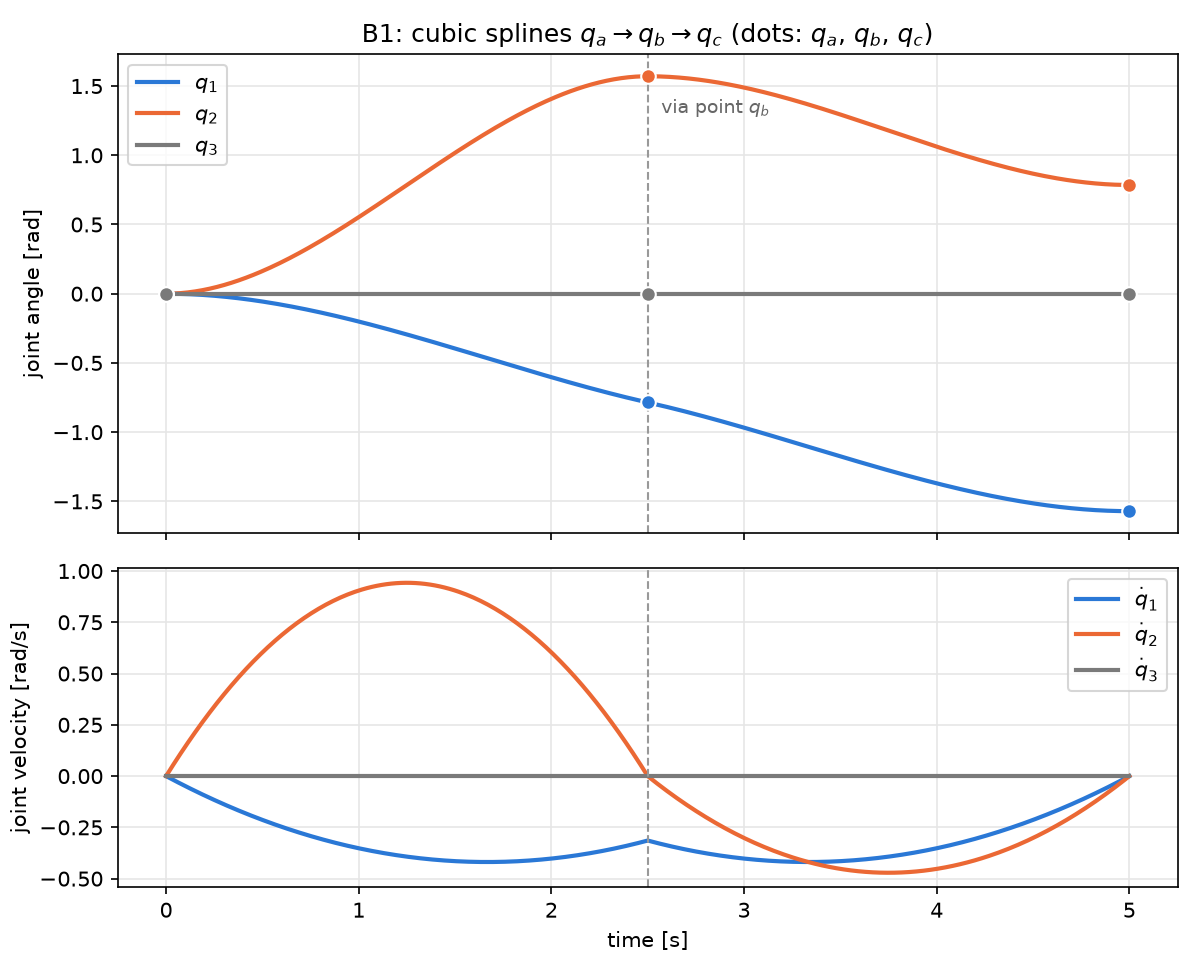
\includegraphics[width=0.75\textwidth]{b1_splines.png}
  \caption{Joint angles (top) and joint velocities (bottom) of the splines from the table. The dots
  are the given configurations $q_a$, $q_b$, $q_c$.}
  \label{fig:b1}
\end{figure}

The splines pass through $q_a$, $q_b$ and $q_c$. The velocity is continuous at the via point: joint 1
passes it with $-0.31$\,rad/s, joint 2 stops there for a moment and turns around.

\subsection*{Task 2: Trajectories in joint space}

\subsubsection*{(a) Trajectory generation}

\texttt{initNjtrackControl()} computes one cubic spline per joint from the current configuration
\texttt{gv.q} to the desired configuration \texttt{gv.qd} and stores it in the global variable
\texttt{spline}:
\[
  q_d(t) = a_0 + a_1 (t - t_0) + a_2 (t - t_0)^2 + a_3 (t - t_0)^3, \qquad t_0 \le t \le t_0 + t_f
\]
The robot starts and ends at rest. With these four conditions the parameters are (tutorial):
\[
  a_0 = q(t_0), \qquad a_1 = 0, \qquad a_2 = \frac{3}{t_f^2}\,(q_d - q(t_0)), \qquad
  a_3 = -\frac{2}{t_f^3}\,(q_d - q(t_0))
\]
$t_0$ is the simulator time \texttt{gv.curTime} when the controller is started.

\textbf{Duration $t_f$.} Velocity and acceleration of the spline are
$\dot q_d(t) = 2 a_2 t + 3 a_3 t^2$ and $\ddot q_d(t) = 2 a_2 + 6 a_3 t$ (with $t$ measured from $t_0$).
The acceleration is a straight line, it is largest at the start and at the end. The velocity is a
parabola, it is largest in the middle at $t = t_f / 2$. With $\Delta q = q_d - q(t_0)$:
\begin{align*}
  |\dot q|_{\max} &= \left|\dot q_d\!\left(\tfrac{t_f}{2}\right)\right| = \frac{3\,|\Delta q|}{2\, t_f} \le \dot q_{\max}
  &&\Rightarrow\quad t_f \ge \frac{3\,|\Delta q|}{2\, \dot q_{\max}} \\
  |\ddot q|_{\max} &= |\ddot q_d(0)| = \frac{6\,|\Delta q|}{t_f^2} \le \ddot q_{\max}
  &&\Rightarrow\quad t_f \ge \sqrt{\frac{6\,|\Delta q|}{\ddot q_{\max}}}
\end{align*}
\texttt{computeTf()} evaluates both bounds for every joint with \texttt{gv.dqmax} and
\texttt{gv.ddqmax} and returns the largest value. This way every joint respects both limits, and
because all joints use the same $t_f$ they reach their goal at the same time.
The helper function \texttt{computeSpline()} calls \texttt{computeTf()} and fills the spline
parameters. It is called from \texttt{initNjtrackControl()}.

\subsubsection*{(b) Control}

In every control cycle \texttt{njtrackControl()} evaluates the spline and its derivative at the current
time and writes them to \texttt{gv.qd} and \texttt{gv.dqd}. The torque is the PD control law with
gravity compensation from the sheet:
\[
  \tau = -k_p\,(q - q_d) - k_v\,(\dot q - \dot q_d) + G(q)
\]
For $G$ we use \texttt{gv.G} computed by the simulator, \texttt{PreprocessControl()} does not overwrite it
any more. After $t_f$ the controller switches to float control ($\tau = G$).

\subsubsection*{(c) Trajectory to a specific point}

\texttt{initProj1Control()} sets \texttt{gv.qd} to $(0.096,\ 0.967,\ -1.061)^T$\,rad and computes the
spline with the same function as in (a). \texttt{proj1Control()} follows it with the controller from (b).

From the zero configuration, with $\dot q_{\max} = 0.79$\,rad/s and $\ddot q_{\max} = 1.05$\,rad/s$^2$
for all joints:

\begin{table}[H]
  \centering
  \caption{Lower bounds for $t_f$ in \texttt{proj1Control}}
  \begin{tabular}{l c c c}
    \toprule
    & Joint 1 & Joint 2 & Joint 3 \\
    \midrule
    $|\Delta q|$ [rad] & 0.10 & 0.97 & 1.06 \\
    $t_f$ from the velocity limit [s] & 0.18 & 1.84 & 2.01 \\
    $t_f$ from the acceleration limit [s] & 0.74 & 2.35 & 2.46 \\
    \bottomrule
  \end{tabular}
\end{table}

The largest value is $t_f = 2.46$\,s (acceleration limit of joint 3). All joints use this duration and
reach the goal at the same time, see Fig.~\ref{fig:proj1}.

\textbf{Gains:} $k_p = [3000,\ 1350,\ 300]^T$, $k_v = [245,\ 70,\ 21]^T$ (for \texttt{njtrack} and
\texttt{proj1}).

The desired position changes smoothly, so the error stays small and $k_p$ can be much higher than for
the step in assignment 1 without exceeding the torque limits. We tuned the gains manually in the
simulator.

\begin{figure}[H]
  \centering
  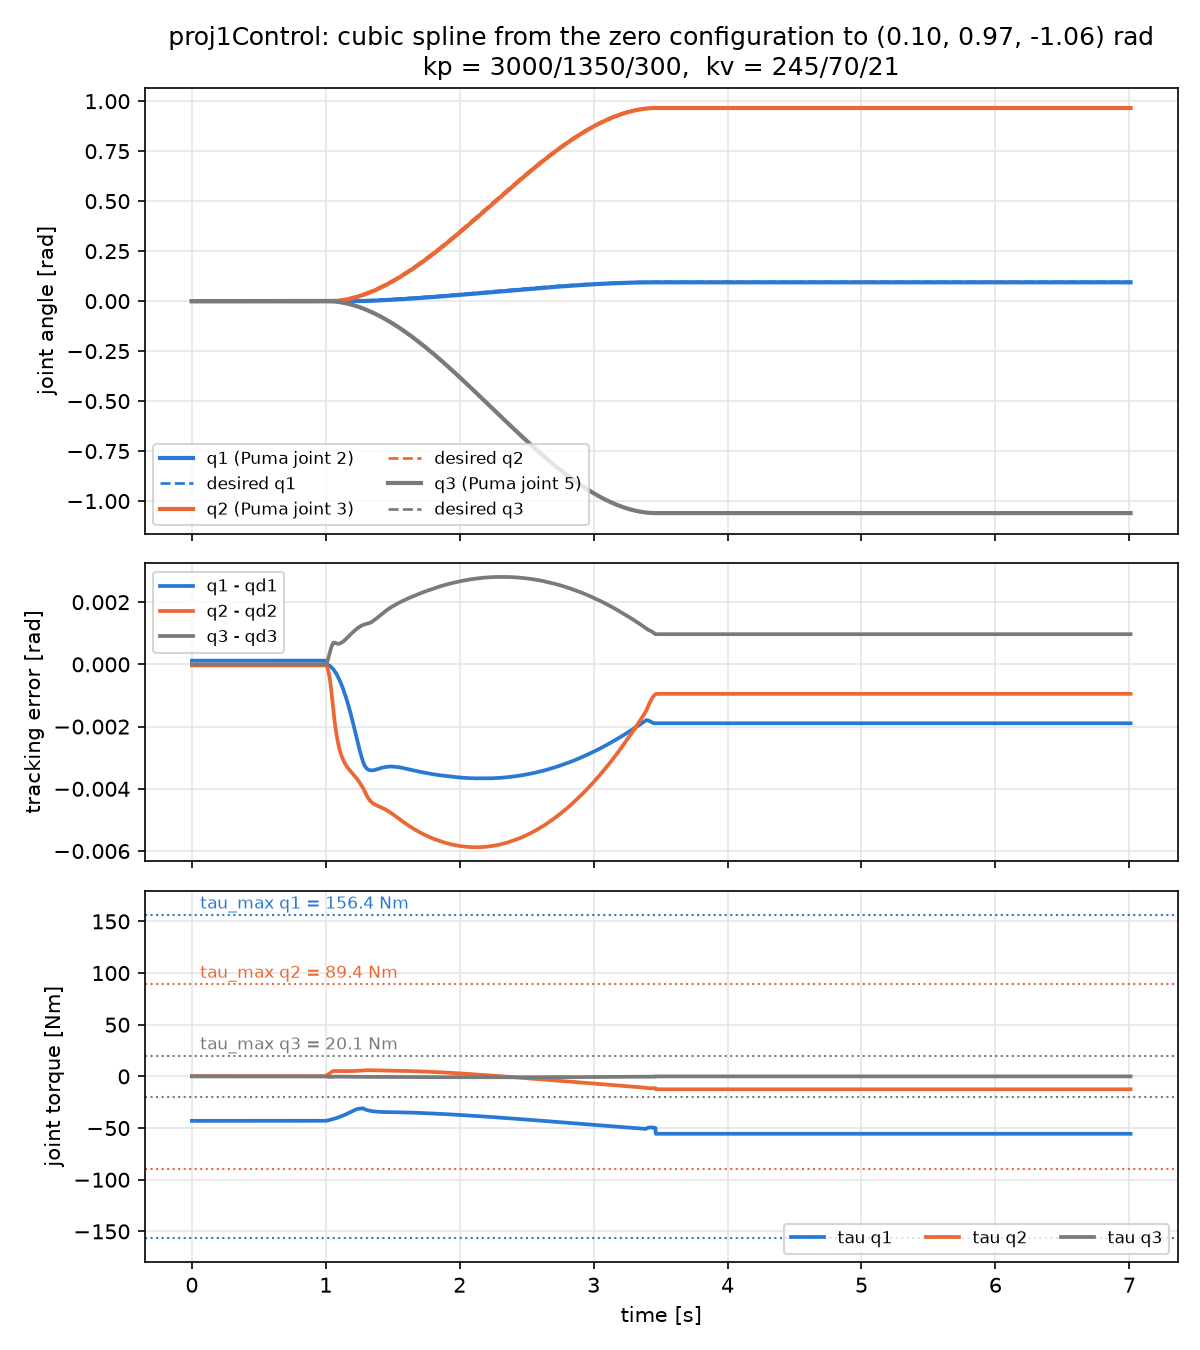
\includegraphics[width=0.78\textwidth]{proj1_track.png}
  \caption{\texttt{proj1Control}: joint angles $q$ and desired angles $q_d$, tracking error and joint
  torques $\tau$. The trajectory starts at $t = 1$\,s. Gains: $k_p = 3000/1350/300$, $k_v = 245/70/21$.}
  \label{fig:proj1}
\end{figure}

The actual and the desired angles lie on top of each other. The tracking error stays below 0.01\,rad
for all joints and the largest torque is 55.5\,Nm at joint 1, far below the limit of 156.4\,Nm. After
$t_f$ the float controller holds the arm, so a small constant error remains.

% ===========================================================================
\section*{C: Operational Space Control}

All quantities of this part are in the simulator frame ($x$ to the right, $y$ up). \texttt{gv.x}
contains $(x, y, \alpha)$ of the end effector, $\alpha = 0$ means upright.

\subsection*{Task 1: Project 2 -- Circle}

The position on the circle is described by the angle $\beta$, measured from the start point around the
center $x_{center} = (0.6,\ 0.35)$\,m with $r = 0.2$\,m. With the constant angular velocity
$\dot\beta = \frac{2\pi}{5}$\,rad/s:
\[
  \beta(t) = \dot\beta\,(t - t_{start})
\]
\[
  x_d = \begin{pmatrix} 0.6 + r \cos\beta \\ 0.35 + r \sin\beta \\ 0 \end{pmatrix},
  \qquad
  \dot x_d = \begin{pmatrix} -r\,\dot\beta \sin\beta \\ r\,\dot\beta \cos\beta \\ 0 \end{pmatrix}
\]
\begin{itemize}
  \item For $\beta = 0$ the position is $(0.8,\ 0.35)$\,m, the required start point.
  \item $\dot x_d$ is the time derivative of $x_d$. The controller needs it for the D-term.
  \item The third component is the desired orientation: it stays 0 (upright), its velocity is 0.
  \item A positive $\beta$ is a rotation about the $z$ axis of the simulator frame. $z$ points out of
        the screen, so on the screen the end effector moves counter-clockwise, as the arrow in Fig.~3 of
        the sheet. Viewed into the positive $z$ direction this is clockwise.
  \item One circle takes $2\pi / \dot\beta = 5$\,s.
\end{itemize}
\texttt{initProj2Control()} stores the start time $t_{start}$ (\texttt{gv.curTime}).
\texttt{proj2Control()} computes $\beta$ and writes $x_d$ and $\dot x_d$ to \texttt{gv.xd} and
\texttt{gv.dxd} (function \texttt{setCircleTarget()}).

\subsection*{Task 2: Project 2 -- Control}

The controller first computes a force (and a torque for the orientation) at the end effector with the
control law of the sheet,
\[
  F = -k_p\,(x - x_d) - k_v\,(\dot x - \dot x_d),
\]
and then maps it to joint torques with the transposed Jacobian and adds the gravity compensation
(lecture):
\[
  \tau = J^T(q)\, F + G(q)
\]
In the code (function \texttt{operationalSpaceControl()}) we use \texttt{gv.x}, \texttt{gv.dx},
\texttt{gv.xd}, \texttt{gv.dxd}, \texttt{gv.Jtranspose} and \texttt{gv.G} from the simulator.
$F$ acts like a spring and a damper that pull the end effector to the desired position. No inverse
kinematics is needed, because the error is computed in operational space and only the resulting force
is transformed to the joints.

\subsection*{Task 3: Project 2 -- Gain tuning and plots}

\textbf{Gains:} $k_p = [8000,\ 8000,\ 200]^T$ and $k_v = [280,\ 280,\ 10]^T$ for $(x, y, \alpha)$.

Before the recording the robot was moved to the start point with \texttt{proj1Control}
($x = (0.80,\ 0.35,\ 0)$).

\begin{figure}[H]
  \centering
  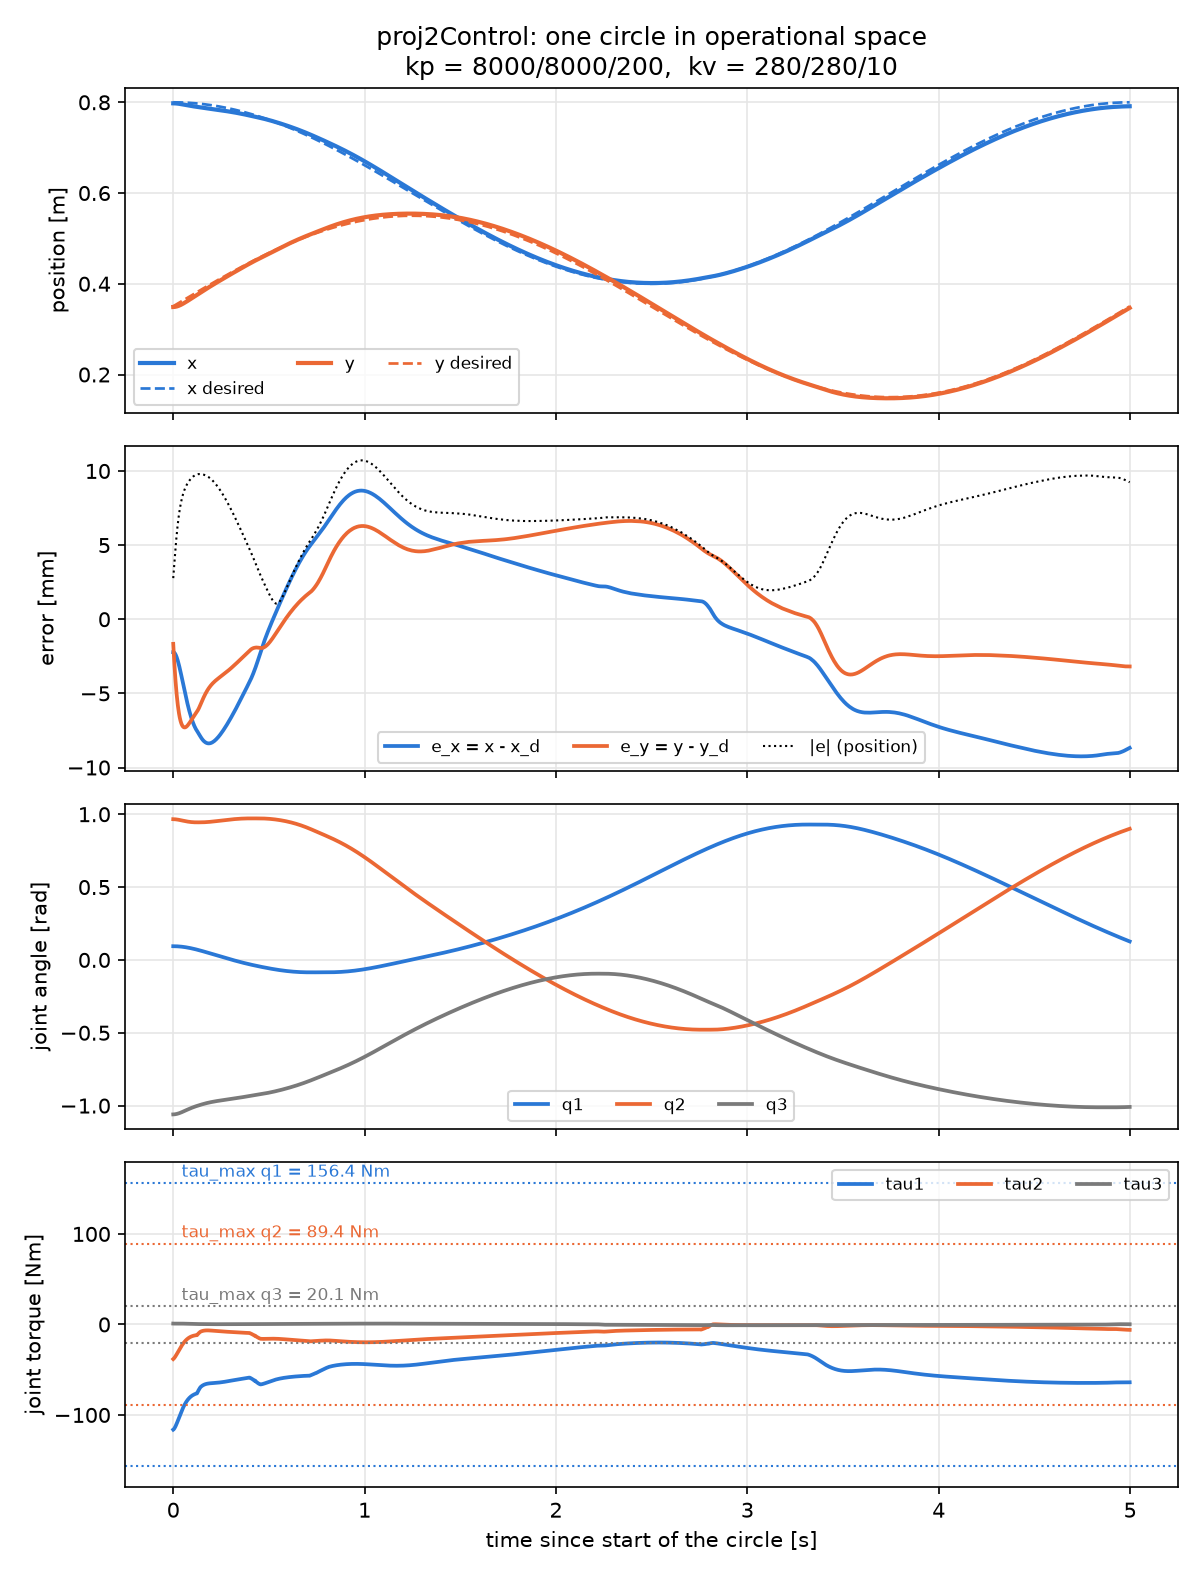
\includegraphics[width=0.78\textwidth]{proj2_circle.png}
  \caption{\texttt{proj2Control}, one circle: position $x$ and desired position $x_d$, position error
  $e = x - x_d$, joint angles $q$ and joint torques $\tau$ (dotted: torque limits).
  Gains: $k_p = 8000/8000/200$, $k_v = 280/280/10$.}
  \label{fig:proj2}
\end{figure}

\begin{figure}[H]
  \centering
  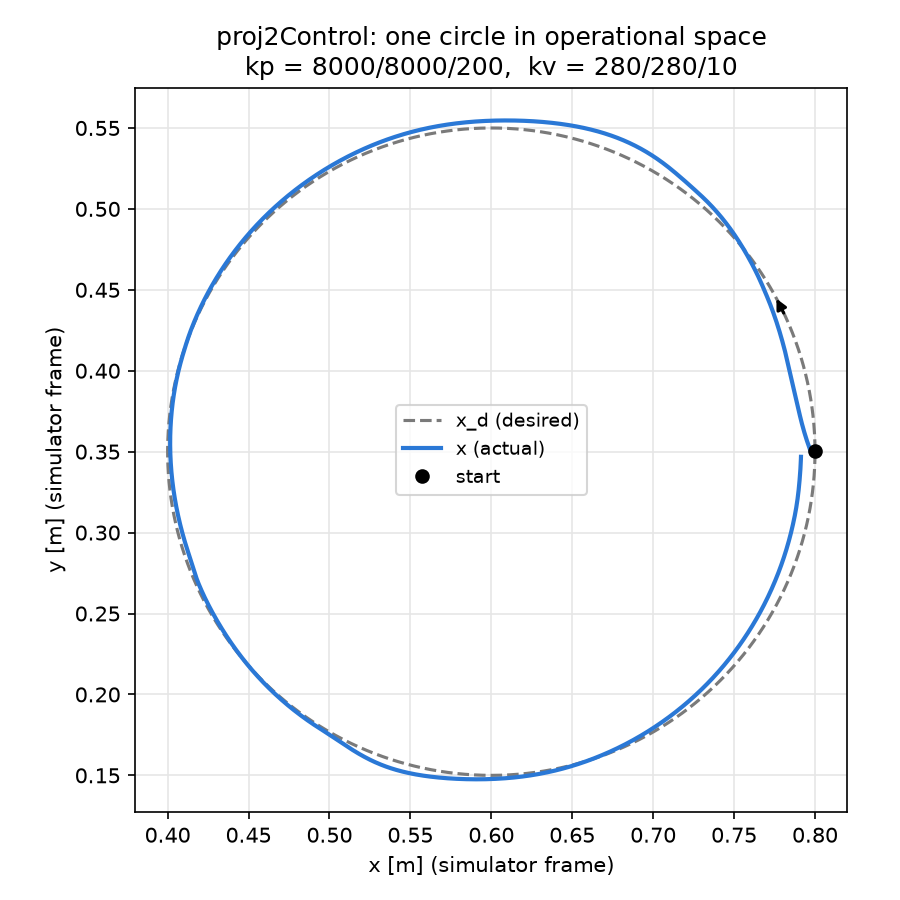
\includegraphics[width=0.55\textwidth]{proj2_xy.png}
  \caption{\texttt{proj2Control}: $x$ and $x_d$ in the $x$-$y$-plane for one circle.
  Gains: $k_p = 8000/8000/200$, $k_v = 280/280/10$.}
  \label{fig:proj2xy}
\end{figure}

With these gains the position error stays below 11\,mm (0.01\,m) during the whole circle and the
orientation error below 0.03\,rad. The torques stay within the limits: the largest values are
116\,Nm at joint 1 (limit 156.4), 38\,Nm at joint 2 (limit 89.4) and 1\,Nm at joint 3 (limit 20.1).

The largest torque occurs directly at the start. The robot is at rest, but the desired velocity jumps
from 0 to $r \dot\beta = 0.25$\,m/s, so the D-term immediately asks for a large force. In
Fig.~\ref{fig:proj2xy} this is visible as the deviation right after the start point.

\textbf{How does the error change for different values of $k_p$?}

\begin{figure}[H]
  \centering
  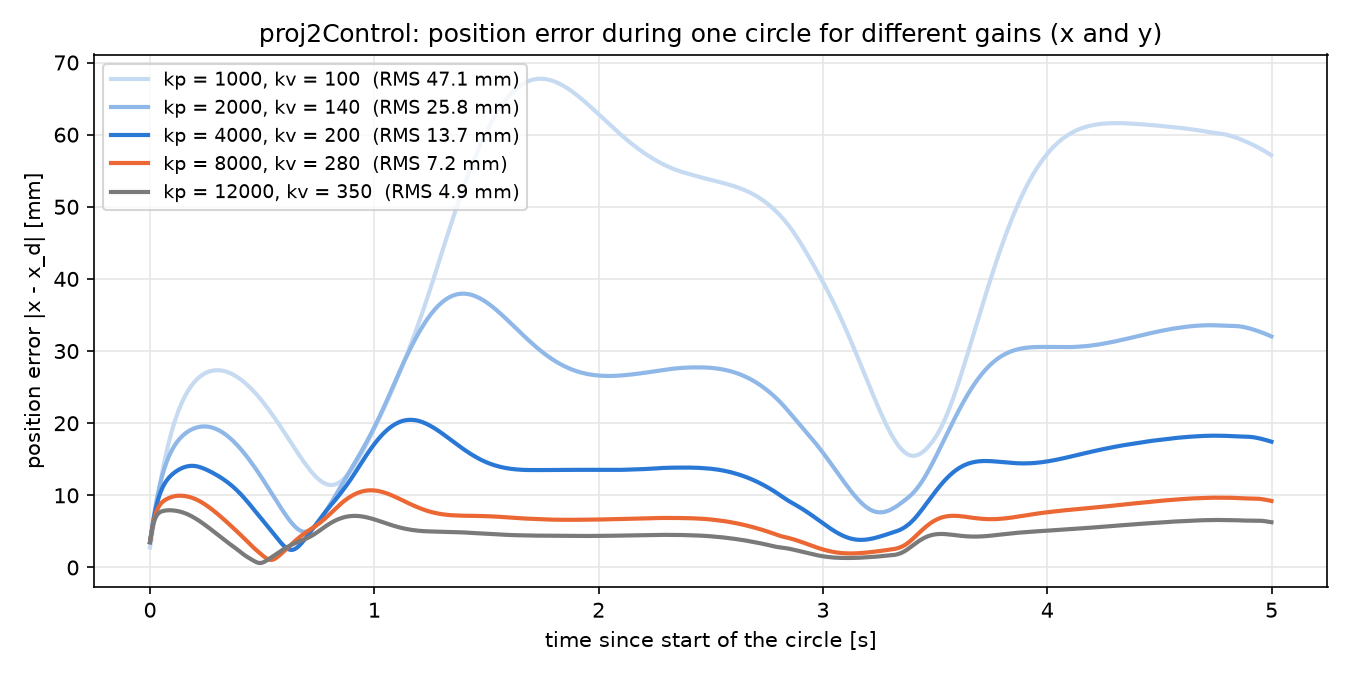
\includegraphics[width=0.85\textwidth]{proj2_error_vs_kp.png}
  \caption{Position error $|x - x_d|$ during one circle for different gains ($k_p$ and $k_v$ for $x$ and
  $y$; orientation gains unchanged).}
  \label{fig:proj2kp}
\end{figure}

The shape of the error curve stays similar, but its size shrinks when $k_p$ grows. Doubling $k_p$
roughly halves the error (RMS error 47\,mm for $k_p = 1000$, 26\,mm for 2000, 14\,mm for 4000, 7\,mm
for 8000). Our explanation: the controller is a spring between $x$ and $x_d$. To move the arm along
the circle a certain force is needed, and a spring with stiffness $k_p$ needs the deflection
$e = F / k_p$ to produce it.

The torque limits bound $k_p$ from above. With $k_p = 12000$ the error is smaller (5\,mm), but the peak
torque at joint 1 is 146\,Nm, which is close to the limit. We therefore chose $k_p = 8000$.
$k_v$ was increased together with $k_p$ so that the end effector does not oscillate around the circle.
A much higher $k_v$ is not possible either: with $k_v = 500$ the jump of the desired velocity at the
start produces 168\,Nm at joint 1.

\subsection*{Task 4: Project 3 -- Parabolic blends}

In \texttt{proj2Control} the desired velocity jumps at the start. \texttt{proj3Control} avoids this with
parabolic blends for the angle $\beta$: the angular velocity first rises linearly (constant
acceleration $\ddot\beta = \frac{2\pi}{25}$\,rad/s$^2$), then stays at
$\dot\beta = \frac{2\pi}{5}$\,rad/s, and finally decreases linearly to 0.

\textbf{Blend time} (hint of the sheet):
\[
  \dot\beta(t_b) = t_b\,\ddot\beta = \frac{2\pi}{5}
  \quad\Rightarrow\quad
  t_b = \frac{\dot\beta}{\ddot\beta} = \frac{2\pi/5}{2\pi/25} = 5\,\text{s}
\]
\textbf{Total time.} During one blend the angle changes by
$\frac{1}{2}\ddot\beta\, t_b^2 = \frac{1}{2}\cdot\frac{2\pi}{25}\cdot 25 = \pi$. Three full circles are
$\beta_f = 6\pi$, so $6\pi - 2\pi = 4\pi$ remain for the linear part, which takes
$4\pi / \dot\beta = 10$\,s. The whole trajectory takes $t_f = 5 + 10 + 5 = 20$\,s.

\textbf{Trajectory} (with $t$ measured from the start):
\[
  \beta(t) =
  \begin{cases}
    \frac{1}{2}\ddot\beta\, t^2 & 0 \le t < t_b \\[3pt]
    \frac{1}{2}\ddot\beta\, t_b^2 + \dot\beta\,(t - t_b) & t_b \le t < t_f - t_b \\[3pt]
    \beta_f - \frac{1}{2}\ddot\beta\,(t_f - t)^2 & t_f - t_b \le t < t_f \\[3pt]
    \beta_f & t \ge t_f
  \end{cases}
  \qquad
  \dot\beta(t) =
  \begin{cases}
    \ddot\beta\, t & 0 \le t < t_b \\[3pt]
    \dot\beta & t_b \le t < t_f - t_b \\[3pt]
    \ddot\beta\,(t_f - t) & t_f - t_b \le t < t_f \\[3pt]
    0 & t \ge t_f
  \end{cases}
\]
The second blend is the mirror image of the first one. Position and velocity are continuous at both
transitions. $\beta$ and $\dot\beta$ are inserted into the circle equations of Task 1, the controller
is the same as in Task 2. After $t_f$ the robot holds the end point. We used the same gains as for
\texttt{proj2}: $k_p = [8000,\ 8000,\ 200]^T$, $k_v = [280,\ 280,\ 10]^T$.

\begin{figure}[H]
  \centering
  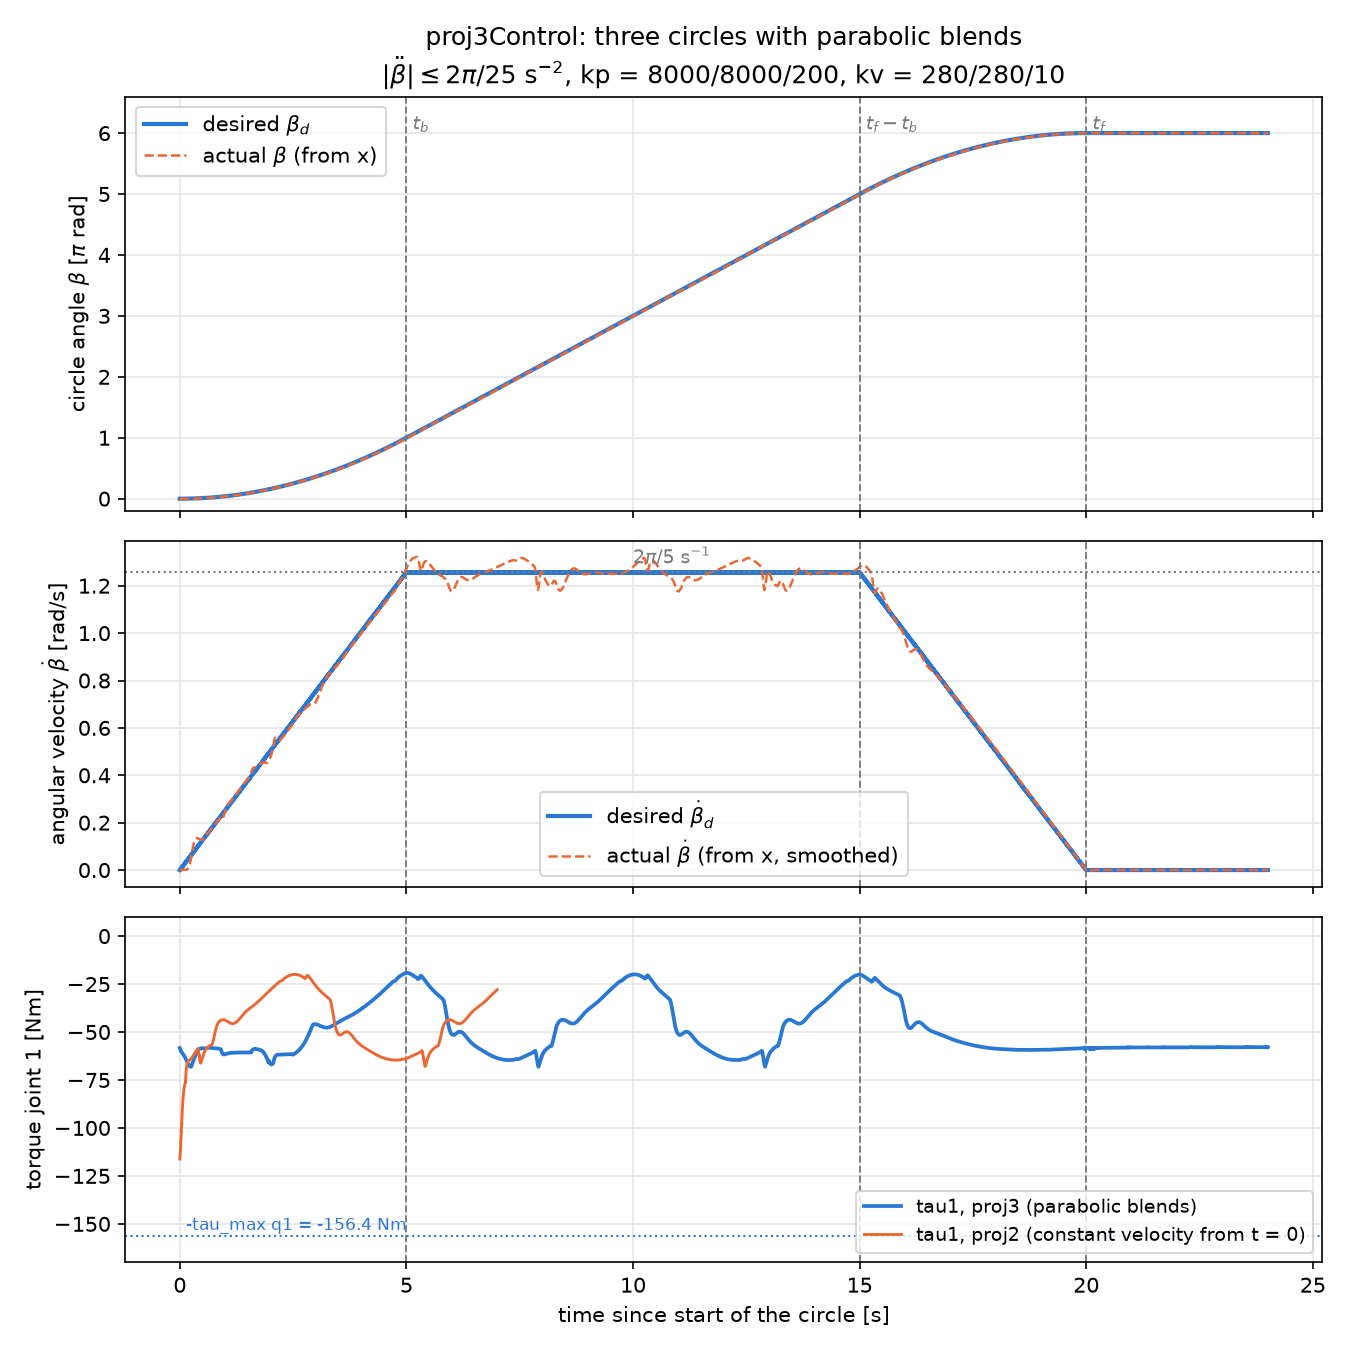
\includegraphics[width=0.78\textwidth]{proj3_blends.png}
  \caption{\texttt{proj3Control}: desired angle $\beta$ and desired angular velocity $\dot\beta$ over
  time for the whole trajectory (blue), together with the measured values (orange, dashed). Bottom:
  torque of joint 1 compared with \texttt{proj2}. Gains: $k_p = 8000/8000/200$, $k_v = 280/280/10$.}
  \label{fig:proj3}
\end{figure}

The position error is again below 11\,mm. Because the velocity no longer jumps, the torque peak at the
start disappears: the largest torque at joint 1 is 68\,Nm instead of 116\,Nm with \texttt{proj2}.

\subsection*{Task 5: Bonus}

For the experiments we used control modes of the template that are not needed otherwise, so that
everything stays in \texttt{control.cpp}. All of them use the operational space controller from Task 2,
the gains of \texttt{proj2} and the same path speed of $r\dot\beta = 0.25$\,m/s.

\subsubsection*{(a) Different trajectories}

\begin{itemize}
  \item \texttt{lineControl}: back and forth on the line from $(0.8,\ 0.35)$ to $(0.4,\ 0.35)$\,m.
  \item \texttt{xtrackControl}: a square with side length 0.2\,m and the corners $(0.8,\ 0.35)$,
        $(0.8,\ 0.55)$, $(0.6,\ 0.55)$, $(0.6,\ 0.35)$\,m.
\end{itemize}

\begin{figure}[H]
  \centering
  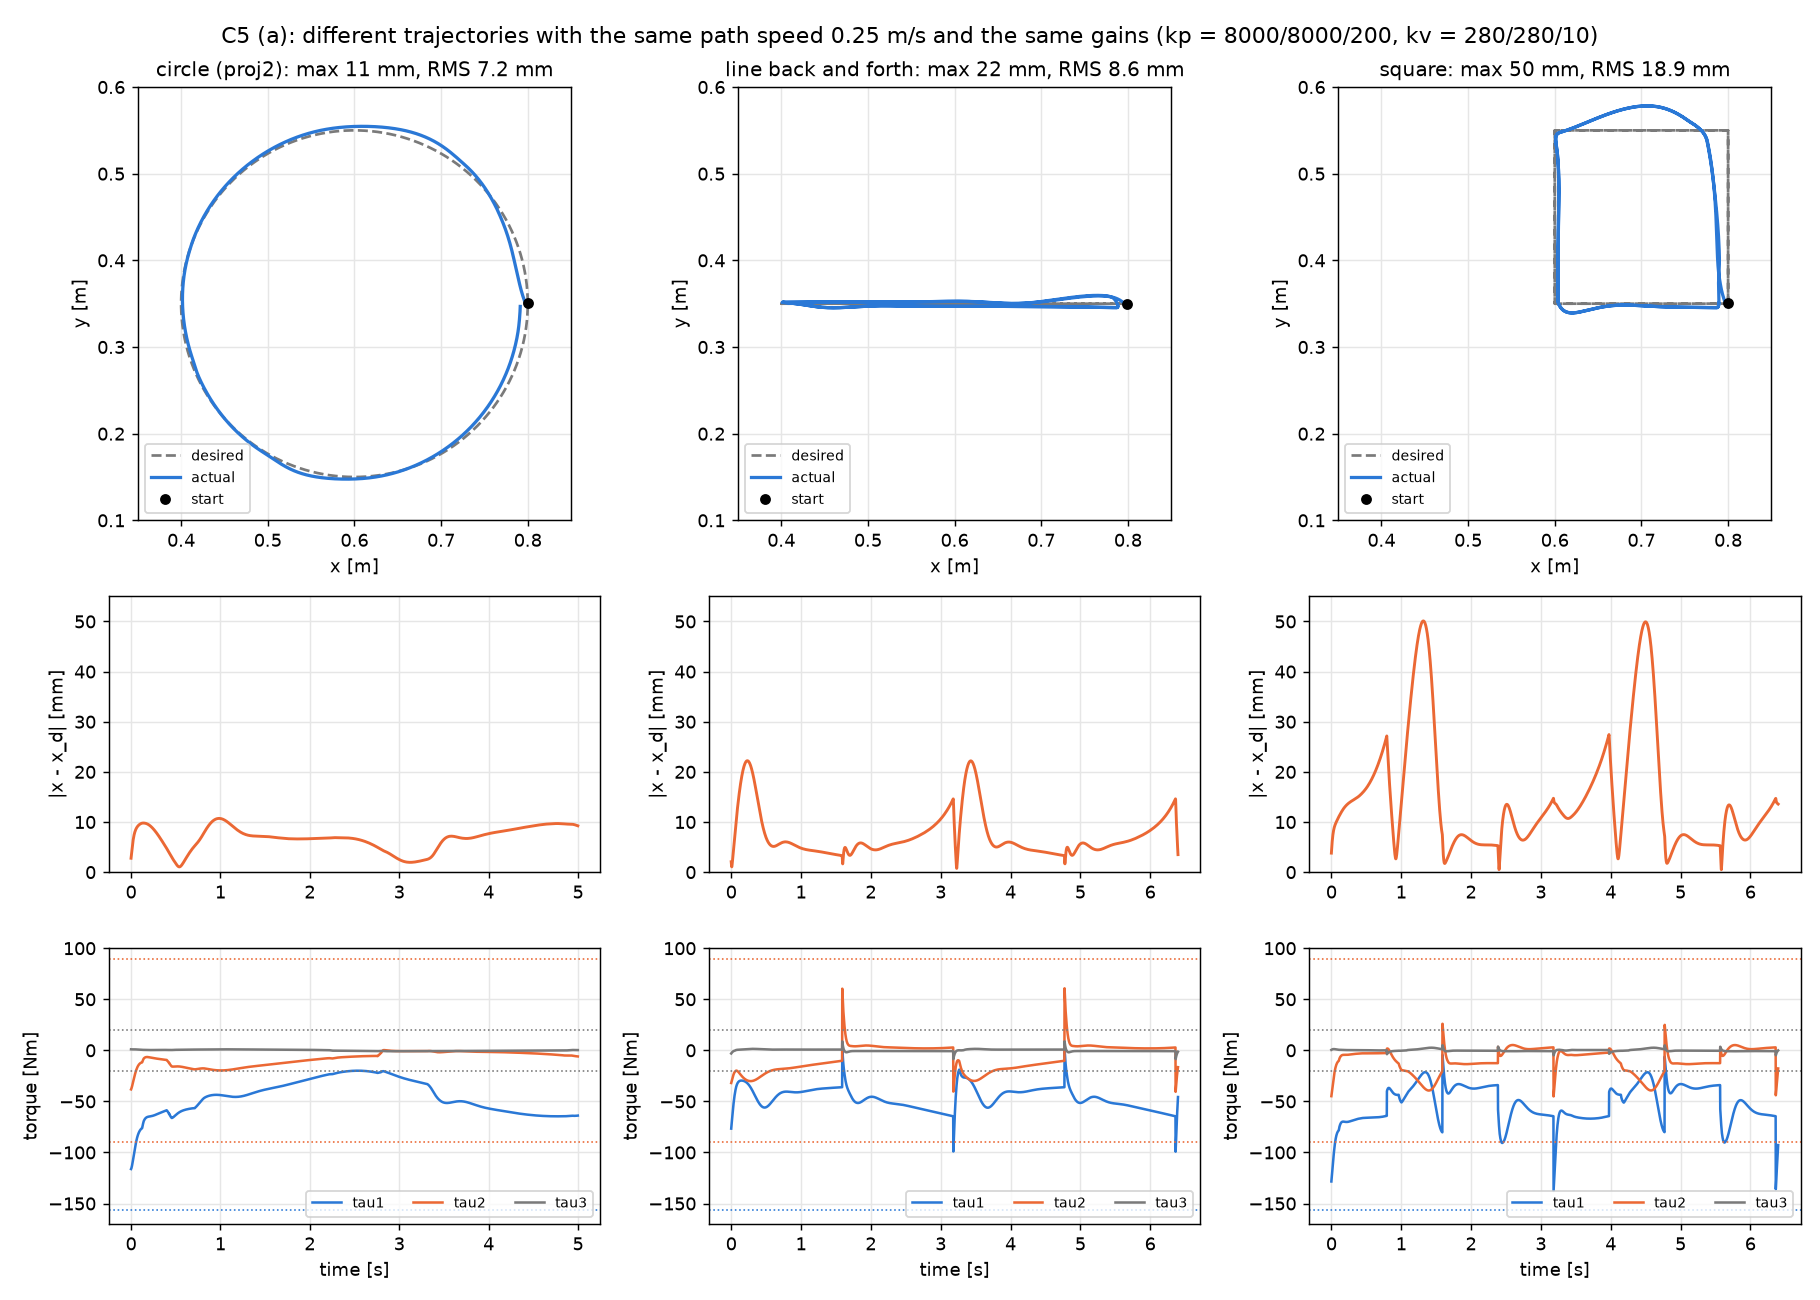
\includegraphics[width=\textwidth]{c5_trajectories.png}
  \caption{Circle, line and square with the same path speed and the same gains
  ($k_p = 8000/8000/200$, $k_v = 280/280/10$). Top: path in the $x$-$y$-plane, middle: position error,
  bottom: joint torques (dotted: torque limits).}
  \label{fig:c5a}
\end{figure}

\begin{table}[H]
  \centering
  \caption{Tracking of the three trajectories (position error $|x - x_d|$)}
  \begin{tabular}{l c c c}
    \toprule
    Trajectory & max. error & RMS error & max. $|\tau_1|$ \\
    \midrule
    Circle & 11\,mm & 7\,mm & 116\,Nm \\
    Line, back and forth & 22\,mm & 9\,mm & 99\,Nm \\
    Square & 50\,mm & 19\,mm & 138\,Nm \\
    \bottomrule
  \end{tabular}
\end{table}

The circle is the easiest to follow. The direction of its velocity changes continuously, so the
required acceleration is finite everywhere. On the straight parts the line and the square are followed
as well as the circle. They are hard at the turning points and at the corners: there the desired
velocity jumps (from $-0.25$ to $+0.25$\,m/s on the line, by a quarter turn at a corner of the square). A
jump in velocity would need an infinite acceleration. The arm overshoots, and the D-term produces a
torque peak. This is the same reason why \texttt{proj3} with parabolic blends needs less torque than
\texttt{proj2}: smooth trajectories are easy, trajectories with jumps in the velocity are hard.

\subsubsection*{(b) Errors and noise in the commanded torques}

Both experiments run the circle of \texttt{proj2} and change the torque after the controller has
computed it:

\begin{itemize}
  \item \texttt{nxtrackControl} (noise): in every control cycle a random value between $-10\,\%$ and
        $+10\,\%$ of $\tau_{\max}$ is added to every joint torque.
  \item \texttt{ntrackControl} (error): only $80\,\%$ of the gravity vector $G$ is compensated.
\end{itemize}

\begin{figure}[H]
  \centering
  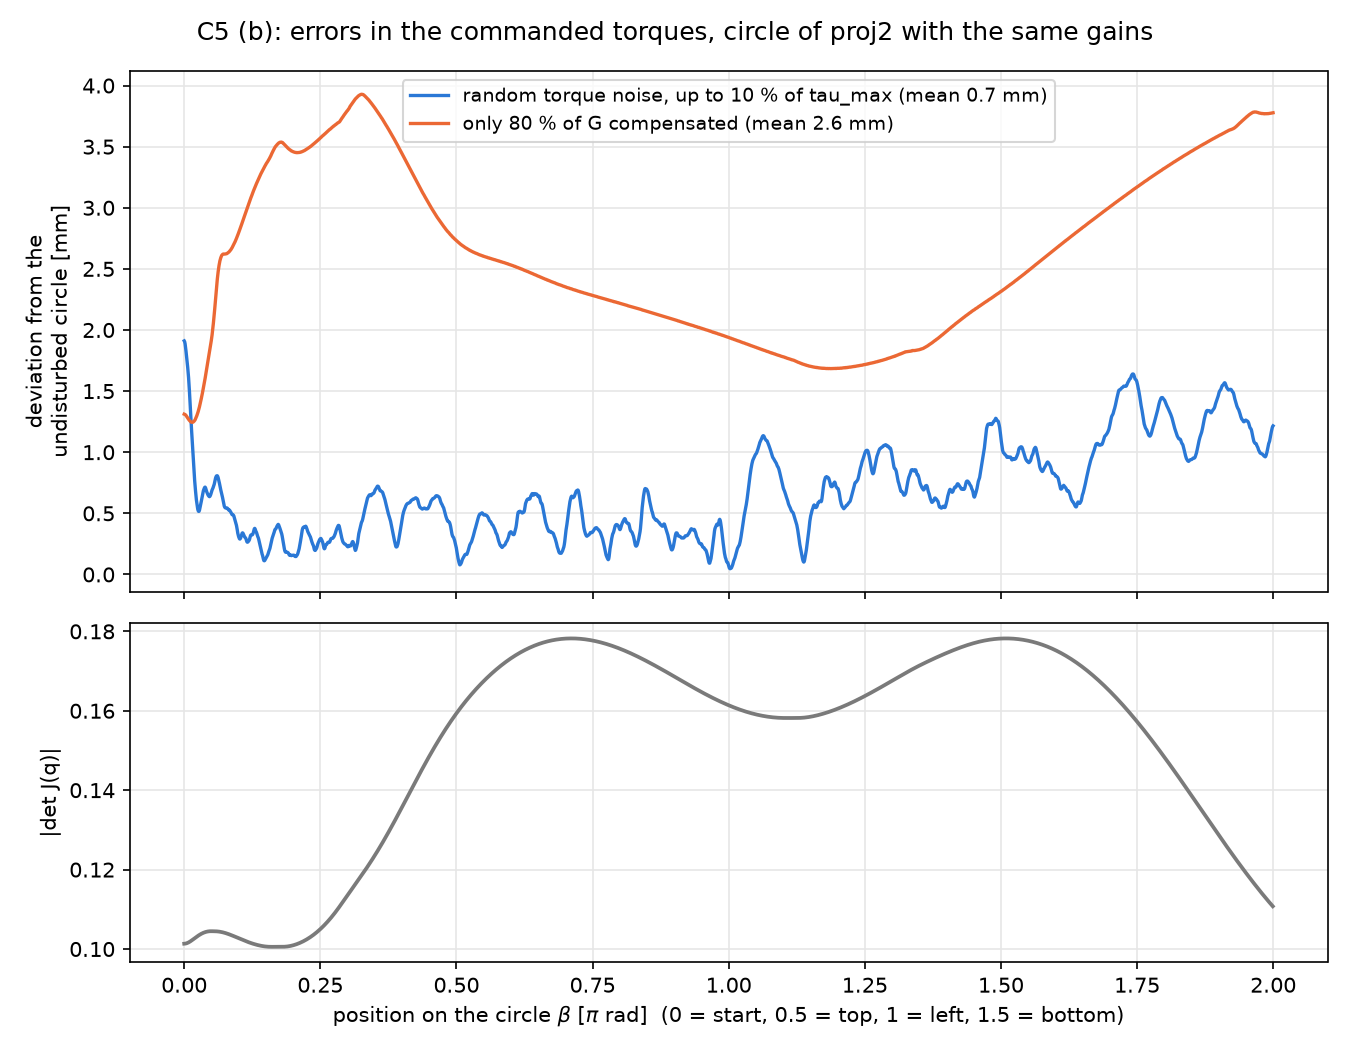
\includegraphics[width=0.78\textwidth]{c5_disturbances.png}
  \caption{Top: distance between the disturbed and the undisturbed circle (\texttt{proj2}) along the
  circle. Bottom: $|\det J(q)|$ along the circle, computed with the Jacobian of part A.}
  \label{fig:c5b}
\end{figure}

\begin{itemize}
  \item \textbf{Noise:} the end effector deviates on average only 0.7\,mm (max. 1.9\,mm) from the
        undisturbed run, although the noise is large (up to 15.6\,Nm at joint 1). The noise changes in
        every control cycle and is zero on average. The inertia of the arm smooths it, and the feedback
        corrects the rest.
  \item \textbf{Error in $G$:} the deviation is larger, on average 2.6\,mm (max. 3.9\,mm). The missing
        torque is always present and always acts in the same direction. The P-term has to provide it, and
        for that it needs a position error.
  \item \textbf{Is the behavior the same across the workspace?} No. For the gravity error the deviation
        changes along the circle between 1.7\,mm and 3.9\,mm. In our run it is large in the first
        quarter and at the end of the circle, where $|\det J|$ is small (about 0.10 to 0.12), i.e. where
        the arm is closer to a singularity. It is small in the middle of the circle, where $|\det J|$ is
        large (about 0.16 to 0.18), see Fig.~\ref{fig:c5b}. Our explanation: the controller compensates a
        torque error with a force $F$ at the end effector, $\tau = J^T F$. Close to a singularity a larger
        force is needed for the same joint torque, and a larger force means a larger error $x - x_d$. In
        addition the missing gravity torque itself depends on the configuration.
\end{itemize}

% ===========================================================================
\section*{Contribution}

\begin{table}[H]
  \centering
  \caption{Contribution Table}
  \begin{tabular}{| l | c | c | c | c | c | c | c | c | c | c | c | c |}
    \hline
    Student Name & (A1) & A2 & A3 & A4 & (A5) & (B1) & B2 & C1 & C2 & C3 & C4 & (C5) \\ \hline
    \hline
    Laurent Stuck     &  &  &  &  &  &  &  &  &  &  &  &  \\ \hline
    \textbf{[name 2]} &  &  &  &  &  &  &  &  &  &  &  &  \\ \hline
    \textbf{[name 3]} &  &  &  &  &  &  &  &  &  &  &  &  \\ \hline
    \textbf{[name 4]} &  &  &  &  &  &  &  &  &  &  &  &  \\ \hline
  \end{tabular}
\end{table}

\end{document}
